% questions.tex —— 2009 年·普通高等学校招生考试·江西卷·文科 · 题目内容片段（无答案）
% 由 tools/generate_projects.py 依来源总账自 2009/2009_数学真题_江西文_试题.md 生成，勿手改（改源 MD 后重跑）


状态：needs-review；依固定候选 PDF 两页（印刷页 535–536）逐题核验，图形已矢量重绘。原页未印分值，不补。

\gkpart{一、选择题}

\begin{question}
\gkti{1}下列命题是真命题的为（　）

（A）若 $\dfrac1x=\dfrac1y$，则 $x=y$

（B）若 $x^2=1$，则 $x=1$

（C）若 $x=y$，则 $\sqrt x=\sqrt y$

（D）若 $x<y$，则 $x^2<y^2$

\end{question}
\begin{question}
\gkti{2}函数 $y=\dfrac{\sqrt{-x^2-3x+4}}{x}$ 的定义域为（　）

（A）$[-4,1]$

（B）$[-4,0)$

（C）$(0,1]$

（D）$[-4,0)\cup(0,1]$

\end{question}
\begin{question}
\gkti{3}$50$ 名学生参加甲、乙两项体育活动，每人至少参加了一项，参加甲项的学生有 $30$ 名，参加乙项的学生有 $25$ 名，则仅参加了一项活动的学生人数为（　）

（A）$50$

（B）$45$

（C）$40$

（D）$35$

\end{question}
\begin{question}
\gkti{4}函数 $f(x)=(1+\sqrt3\tan x)\cos x$ 的最小正周期为（　）

（A）$2\pi$

（B）$\frac{3\pi}{2}$

（C）$\pi$

（D）$\frac{\pi}{2}$

\end{question}
\begin{question}
\gkti{5}已知函数 $f(x)$ 是 $(-\infty,+\infty)$ 上的偶函数，若对于 $x\geqslant0$，都有 $f(x+2)=f(x)$，且当 $x\in[0,2)$ 时，$f(x)=\log_2(x+1)$，则 $f(-2008)+f(2009)$ 的值为（　）

（A）$-2$

（B）$-1$

（C）$1$

（D）$2$

\end{question}
\begin{question}
\gkti{6}若 $\mathrm C_n^1x+\mathrm C_n^2x^2+\cdots+\mathrm C_n^nx^n$ 能被 $7$ 整除，则 $x$，$n$ 的值可能为（　）

（A）$x=4$，$n=3$

（B）$x=4$，$n=4$

（C）$x=5$，$n=4$

（D）$x=6$，$n=5$

\end{question}
\begin{question}
\gkti{7}设 $F_1$ 和 $F_2$ 为双曲线 $\dfrac{x^2}{a^2}-\dfrac{y^2}{b^2}=1$（$a>0$，$b>0$）的两个焦点，若 $F_1$，$F_2$，$P(0,2b)$ 是正三角形的三个顶点，则双曲线的离心率为（　）

（A）$\frac32$

（B）$2$

（C）$\frac52$

（D）$3$

\end{question}
\begin{question}
\gkti{8}公差不为零的等差数列 $\{a_n\}$ 的前 $n$ 项和为 $S_n$．若 $a_4$ 是 $a_3$ 与 $a_7$ 的等比中项，$S_8=32$，则 $S_{10}$ 等于（　）

（A）$18$

（B）$24$

（C）$60$

（D）$90$

\Needspace{0.4\textheight}
\end{question}
\begingroup
\renewenvironment{question}{\Needspace{0.5\textheight}}{}
\begin{question}
\gkti{9}如图，在四面体 $ABCD$ 中，截面 $PQMN$ 是正方形，则在下列命题中，错误的为（　）

（A）$AC\perp BD$

（B）$AC\parallel$ 截面 $PQMN$

（C）$AC=BD$

（D）异面直线 $PM$ 与 $BD$ 所成的角为 $45^\circ$
\nopagebreak[4]
\begin{center}% 2009 年江西卷文科第 9 题：四面体 ABCD 与正方形截面 PQMN。
% 来源 PDF：普通高考/2009/2009江西文.pdf，SHA-256 468ed0d312446a29e8cdaebe70fab4f803741b0b542cd991781b2f13fed5168f。
% 原页：第 1 页（A3 三栏）第 1 栏，书页码 535。
% 重绘依据：原图 A 在顶点，B 在左下、C 在右下，D 在四边形内部（被遮挡，连 AD、BD、CD 为虚线）；
%   截面四顶点 P∈AB、N∈AD、M∈DC、Q∈BC，PQ∥AC、PN∥BD，取 AP/AB=0.59、BQ/BC=0.41 使投影两侧近似等长。
%   原图 P-N、P-Q 为实线，N-M、M-Q 为虚线。
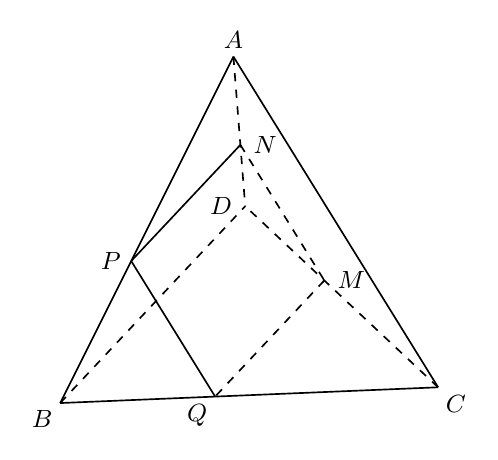
\begin{tikzpicture}[scale=1.0, semithick, every node/.style={inner sep=1.5pt, font=\small}]
  \coordinate (A) at (0,4.40);
  \coordinate (B) at (-2.20,0);
  \coordinate (C) at (2.60,0.20);
  \coordinate (D) at (0.15,2.50);
  \coordinate (P) at (-1.298,1.804);
  \coordinate (Q) at (-0.232,0.082);
  \coordinate (N) at (0.0885,3.279);
  \coordinate (M) at (1.1545,1.557);

  % 四面体的棱：实线为可见棱，虚线为被遮挡棱
  \draw (A) -- (B);
  \draw (A) -- (C);
  \draw (B) -- (C);
  \draw[dashed] (A) -- (D);
  \draw[dashed] (B) -- (D);
  \draw[dashed] (C) -- (D);

  % 正方形截面 PQMN：靠前的两条边实线，靠后的两条边虚线
  \draw (P) -- (N);
  \draw (P) -- (Q);
  \draw[dashed] (N) -- (M);
  \draw[dashed] (M) -- (Q);

  \node[above=1pt] at (A) {$A$};
  \node[below left=1pt] at (B) {$B$};
  \node[below right=1pt] at (C) {$C$};
  \node[left=2pt] at (P) {$P$};
  \node[below left=1pt] at (Q) {$Q$};
  \node[right=3pt] at (N) {$N$};
  \node[right=3pt] at (M) {$M$};
  \node[left=3pt] at (D) {$D$};
\end{tikzpicture}
\end{center}
\nopagebreak[4]
\end{question}
\endgroup
\begin{question}
\gkti{10}甲、乙、丙、丁 $4$ 个足球队参加比赛，假设每场比赛各队取胜的概率相等，现任意将这 $4$ 个队分成两个组（每组两个队）进行比赛，胜者再赛．则甲、乙相遇的概率为（　）

（A）$\frac16$

（B）$\frac14$

（C）$\frac13$

（D）$\frac12$

\Needspace{0.4\textheight}
\end{question}
\begingroup
\renewenvironment{question}{\Needspace{0.5\textheight}}{}
\begin{question}
\gkti{11}如图所示，一质点 $P(x,y)$ 在 $xOy$ 平面上沿曲线运动，速度大小不变，其在 $x$ 轴上的投影点 $Q(x,0)$ 的运动速度 $V=V(t)$ 的图象大致为（　）
\nopagebreak[4]
\begin{center}% 2009 年江西卷文科第 11 题：（上）质点轨迹与投影点 Q，（下）四个候选 V(t) 图象。
% 来源 PDF：普通高考/2009/2009江西文.pdf，SHA-256 468ed0d312446a29e8cdaebe70fab4f803741b0b542cd991781b2f13fed5168f。
% 原页：第 1 页（A3 三栏）第 2 栏，书页码 535。
% 重绘依据：原图轨迹自 y 轴出发沿直线上升至折点，随后展平并依次形成一大一小两个闭合环，末端变陡上升；
%   四个选项按原图特征区分：(A) 始终非负、两次触及 t 轴；(B) 起点为常数、折点处上跳、两次出现负值、末端下降；
%   (C) 起点为斜线（非常数）；(D) 起点常数、上跳后两次出现负值、末端上升。
\begin{tikzpicture}[semithick, every node/.style={inner sep=1.3pt, font=\small}]

  %========== 轨迹图 ==========
  \begin{scope}[shift={(0,3.62)}, x=0.80cm, y=0.80cm]
    \draw[-{Stealth}] (-0.55,0) -- (7.15,0) node[right] {$x$};
    \draw[-{Stealth}] (0,-0.25) -- (0,3.30) node[above] {$y$};
    \node[below left=2pt] at (0,0) {$O$};
    % 轨迹：直线上升 -> 折点 -> 展平 -> 大环 -> 小环 -> 末端变陡
    \draw (0,1.15) -- (1.30,2.90)
      .. controls (1.55,2.30) and (1.72,1.70) .. (2.10,1.35)
      .. controls (2.45,1.05) and (2.85,0.95) .. (3.15,1.00)
      .. controls (3.45,1.03) and (3.62,1.08) .. (3.80,1.16)
      .. controls (4.15,1.28) and (4.55,1.20) .. (4.80,1.02)
      .. controls (4.98,0.90) and (5.12,0.95) .. (5.28,1.08)
      .. controls (5.50,1.28) and (5.68,1.60) .. (5.85,1.95)
      .. controls (6.02,2.30) and (6.20,2.55) .. (6.42,2.80);
    % 大环
    \draw (3.80,1.16)
      .. controls (3.32,1.26) and (3.05,1.75) .. (3.18,2.20)
      .. controls (3.30,2.65) and (3.75,3.00) .. (4.12,2.95)
      .. controls (4.50,2.90) and (4.68,2.45) .. (4.55,2.05)
      .. controls (4.42,1.65) and (4.10,1.28) .. (3.80,1.16);
    % 小环
    \draw (5.28,1.08)
      .. controls (5.02,1.18) and (4.98,1.60) .. (5.14,1.92)
      .. controls (5.30,2.24) and (5.62,2.30) .. (5.80,2.05)
      .. controls (5.98,1.80) and (5.86,1.40) .. (5.60,1.20)
      .. controls (5.50,1.14) and (5.38,1.10) .. (5.28,1.08);
    % 投影点 Q 与虚线
    \draw[dashed] (2.10,1.35) -- (2.10,0);
    \node[below=1pt] at (2.10,0) {$Q(x,0)$};
    \node[anchor=east] at (2.02,0.80) {$P(x,y)$};
  \end{scope}

  %========== (A) ==========
  \begin{scope}[shift={(0.35,-0.30)}, x=0.60cm, y=0.60cm]
    \draw[-{Stealth}] (-0.15,0) -- (4.75,0) node[right] {$t$};
    \draw[-{Stealth}] (0,-0.30) -- (0,2.35) node[above] {$V(t)$};
    \node[below left=1pt] at (0,0) {$O$};
    \draw (0,1.00) -- (1.45,1.00)
      .. controls (1.65,1.00) and (1.70,1.45) .. (1.85,1.72)
      -- (2.25,1.72)
      .. controls (2.50,1.72) and (2.58,0.95) .. (2.80,0.00)
      .. controls (2.92,0.00) and (3.00,0.55) .. (3.16,1.30)
      .. controls (3.28,1.85) and (3.34,2.05) .. (3.50,2.06)
      .. controls (3.68,2.06) and (3.74,1.20) .. (3.94,0.00)
      .. controls (4.06,0.00) and (4.14,0.60) .. (4.28,1.35)
      .. controls (4.40,2.00) and (4.52,2.10) .. (4.66,1.90);
    \node at (1.55,-0.95) {(A)};
  \end{scope}

  %========== (B) ==========
  \begin{scope}[shift={(5.00,-0.30)}, x=0.60cm, y=0.60cm]
    \draw[-{Stealth}] (-0.15,0) -- (5.60,0) node[right] {$t$};
    \draw[-{Stealth}] (0,-1.55) -- (0,2.35) node[above] {$V(t)$};
    \node[below left=1pt] at (0,0) {$O$};
    \draw (0,1.05) -- (1.32,1.05)
      .. controls (1.42,1.05) and (1.44,1.72) .. (1.55,1.88)
      -- (1.92,1.88)
      .. controls (2.16,1.88) and (2.24,0.60) .. (2.46,-0.90)
      .. controls (2.62,-2.00) and (2.86,-2.00) .. (3.02,-0.90)
      .. controls (3.20,0.60) and (3.28,1.88) .. (3.50,1.90)
      .. controls (3.72,1.92) and (3.80,0.60) .. (4.00,-0.90)
      .. controls (4.16,-2.00) and (4.40,-2.00) .. (4.56,-0.90)
      .. controls (4.74,0.60) and (4.82,1.88) .. (5.02,1.90)
      .. controls (5.22,1.92) and (5.32,1.55) .. (5.45,1.05);
    \node at (1.20,-1.55) {(B)};
  \end{scope}

  %========== (C) ==========
  \begin{scope}[shift={(0.35,-3.55)}, x=0.60cm, y=0.60cm]
    \draw[-{Stealth}] (-0.15,0) -- (5.05,0) node[right] {$t$};
    \draw[-{Stealth}] (0,-1.55) -- (0,2.35) node[above] {$V(t)$};
    \node[below left=1pt] at (0,0) {$O$};
    \draw (0,0.55) -- (1.55,1.62)
      .. controls (1.85,1.85) and (2.05,1.90) .. (2.25,1.85)
      .. controls (2.52,1.78) and (2.62,0.60) .. (2.85,-0.85)
      .. controls (3.00,-1.95) and (3.22,-1.95) .. (3.38,-0.85)
      .. controls (3.54,0.55) and (3.62,1.85) .. (3.85,1.88)
      .. controls (4.06,1.90) and (4.14,0.60) .. (4.34,-0.85)
      .. controls (4.48,-1.90) and (4.66,-1.90) .. (4.82,-1.05);
    \node at (1.10,-1.60) {(C)};
  \end{scope}

  %========== (D) ==========
  \begin{scope}[shift={(5.00,-3.55)}, x=0.60cm, y=0.60cm]
    \draw[-{Stealth}] (-0.15,0) -- (5.60,0) node[right] {$t$};
    \draw[-{Stealth}] (0,-1.55) -- (0,2.35) node[above] {$V(t)$};
    \node[below left=1pt] at (0,0) {$O$};
    \draw (0,1.05) -- (1.30,1.05)
      .. controls (1.55,1.05) and (1.58,1.80) .. (1.80,1.90)
      -- (2.15,1.90)
      .. controls (2.30,1.90) and (2.36,0.60) .. (2.58,-0.90)
      .. controls (2.74,-2.00) and (2.96,-2.00) .. (3.12,-0.90)
      .. controls (3.30,0.60) and (3.38,1.88) .. (3.60,1.90)
      .. controls (3.82,1.92) and (3.90,0.60) .. (4.10,-0.90)
      .. controls (4.24,-1.90) and (4.44,-1.95) .. (4.62,-0.80);
    \node at (1.20,-1.60) {(D)};
  \end{scope}

\end{tikzpicture}
\end{center}
\nopagebreak[4]
\end{question}
\endgroup
\begin{question}
\gkti{12}若存在过点 $(1,0)$ 的直线与曲线 $y=x^3$ 和 $y=ax^2+\frac{15}{4}x-9$ 都相切，则 $a$ 等于（　）

（A）$-1$ 或 $-\frac{25}{64}$

（B）$-1$ 或 $\frac{21}{4}$

（C）$-\frac74$ 或 $-\frac{25}{64}$

（D）$-\frac74$ 或 $7$

\end{question}
\gkpart{二、填空题}

\begin{question}
\gkti{13}已知向量 $\boldsymbol a=(3,1)$，$\boldsymbol b=(1,3)$，$\boldsymbol c=(k,2)$．若 $(\boldsymbol a-\boldsymbol c)\perp\boldsymbol b$，则 $k=$\gkblank{}．

\end{question}
\begin{question}
\gkti{14}体积为 $8$ 的一个正方体，其全面积与球 $O$ 的表面积相等，则球 $O$ 的体积等于\gkblank{}．

\end{question}
\begin{question}
\gkti{15}若不等式 $\sqrt{4-x^2}\leqslant k(x+1)$ 的解集为区间 $[a,b]$，且 $b-a=1$，则 $k=$\gkblank{}．

\end{question}
\begin{question}
\gkti{16}设直线系 $M$：$x\cos\theta+(y-2)\sin\theta=1$（$0\leqslant\theta\leqslant2\pi$），对于下列四个命题：

\textbf{A．}存在一个圆与所有直线相交；

\textbf{B．}存在一个圆与所有直线不相交；

\textbf{C．}存在一个圆与所有直线相切；

\textbf{D．}$M$ 中的直线所能围成的正三角形面积都相等．

其中真命题的代号是\gkblank{}．（写出所有真命题的代号）

\end{question}
\gkpart{三、解答题}

\begin{question}
\gkti{17}设函数 $f(x)=x^3-\dfrac92x^2+6x-a$．

（1）对于任意实数 $x$，$f'(x)\geqslant m$ 恒成立，求 $m$ 的最大值；

（2）若方程 $f(x)=0$ 有且仅有一个实根，求 $a$ 的取值范围．

\end{question}
\begin{question}
\gkti{18}某公司拟资助三位大学生自主创业，现聘请两位专家，独立地对每位大学生的创业方案进行评审．假设评审结果为“支持”或“不支持”的概率都是 $\dfrac12$．若某人获得两个“支持”，则给予 $10$ 万元的创业资助；若只获得一个“支持”，则给予 $5$ 万元的资助；若未获得“支持”，则不予资助．求：

（1）该公司的资助总额为零的概率；

（2）该公司的资助总额超过 $15$ 万元的概率．

\end{question}
\begin{question}
\gkti{19}$\triangle ABC$ 中，$A$，$B$，$C$ 所对的边分别为 $a$，$b$，$c$，$A=\dfrac{\pi}{6}$，$(1+\sqrt3)c=2b$．

（1）求 $C$；

（2）若 $\overrightarrow{CB}\cdot\overrightarrow{CA}=1+\sqrt3$，求 $a$，$b$，$c$．

\Needspace{0.4\textheight}
\end{question}
\begingroup
\renewenvironment{question}{\Needspace{0.5\textheight}}{}
\begin{question}
\gkti{20}在四棱锥 $P-ABCD$ 中，底面 $ABCD$ 是矩形，$PA\perp$ 平面 $ABCD$，$PA=AD=4$，$AB=2$．以 $BD$ 的中点 $O$ 为球心、$BD$ 为直径的球面交 $PD$ 于点 $M$．

（1）求证：平面 $ABM\perp$ 平面 $PCD$；

（2）求直线 $PC$ 与平面 $ABM$ 所成的角；

（3）求点 $O$ 到平面 $ABM$ 的距离．
\nopagebreak[4]
\begin{center}% 2009 年江西卷文科第 20 题：四棱锥 P-ABCD，球心 O 为 BD 中点，球面交 PD 于 M。
% 来源 PDF：普通高考/2009/2009江西文.pdf，SHA-256 468ed0d312446a29e8cdaebe70fab4f803741b0b542cd991781b2f13fed5168f。
% 原页：第 2 页（A3 三栏）第 1 栏，书页码 536。
% 重绘依据：原图 P 在顶点，B 在左下、C 在右下、D 在右、A 在左后被遮挡；
%   PA、AB、AD、BD、AM、BM 为虚线，PB、PC、PD、BC、CD 为实线，O 为 BD 上的实心点，M 在 PD 上。
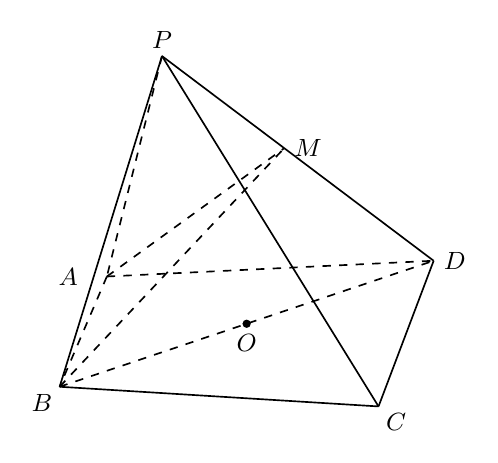
\begin{tikzpicture}[scale=1.0, semithick, every node/.style={inner sep=1.4pt, font=\small}]
  \coordinate (P) at (2.15,5.15);
  \coordinate (A) at (1.45,2.35);
  \coordinate (B) at (0.85,0.95);
  \coordinate (C) at (4.90,0.70);
  \coordinate (D) at (5.60,2.55);
  \coordinate (O) at (3.225,1.75);
  \coordinate (M) at (3.7025,3.98);

  % 可见棱
  \draw (P) -- (B);
  \draw (P) -- (C);
  \draw (P) -- (M) -- (D);
  \draw (B) -- (C);
  \draw (C) -- (D);

  % 被遮挡的棱与辅助线
  \draw[dashed] (P) -- (A);
  \draw[dashed] (A) -- (B);
  \draw[dashed] (A) -- (D);
  \draw[dashed] (B) -- (D);
  \draw[dashed] (A) -- (M);
  \draw[dashed] (B) -- (M);

  % 球心 O
  \fill (O) circle (1.5pt);

  \node[above=1pt] at (P) {$P$};
  \node[anchor=east] at (1.14,2.34) {$A$};
  \node[below left=1pt] at (B) {$B$};
  \node[below right=1pt] at (C) {$C$};
  \node[right=2pt] at (D) {$D$};
  \node[below=2pt] at (O) {$O$};
  \node[right=2pt] at (M) {$M$};
\end{tikzpicture}
\end{center}
\nopagebreak[4]
\end{question}
\endgroup
\begin{question}
\gkti{21}数列 $\{a_n\}$ 的通项 $a_n=n^2\left(\cos^2\dfrac{n\pi}{3}-\sin^2\dfrac{n\pi}{3}\right)$，其前 $n$ 项和为 $S_n$．

（1）求 $S_n$；

（2）$b_n=\dfrac{S_{3n}}{n\cdot4^n}$，求数列 $\{b_n\}$ 的前 $n$ 项和 $T_n$．

\Needspace{0.4\textheight}
\end{question}
\begingroup
\renewenvironment{question}{\Needspace{0.5\textheight}}{}
\begin{question}
\gkti{22}如图，已知圆 $G$：$(x-2)^2+y^2=r^2$ 是椭圆 $\dfrac{x^2}{16}+y^2=1$ 的内接 $\triangle ABC$ 的内切圆，其中 $A$ 为椭圆的左顶点．

（1）求圆 $G$ 的半径 $r$；

（2）过点 $M(0,1)$ 作圆 $G$ 的两条切线交椭圆于 $E$，$F$ 两点，证明：直线 $EF$ 与圆 $G$ 相切．
\nopagebreak[4]
\begin{center}% 2009 年江西卷文科第 22 题：椭圆 x^2/16+y^2=1 的内接三角形 ABC 及其内切圆 G。
% 来源 PDF：普通高考/2009/2009江西文.pdf，SHA-256 468ed0d312446a29e8cdaebe70fab4f803741b0b542cd991781b2f13fed5168f。
% 原页：第 2 页（A3 三栏）第 3 栏，书页码 536。
% 重绘依据：按真实坐标等比绘制（x、y 同尺度）：A(-4,0)，B(8/3,√5/3)，C(8/3,-√5/3)，
%   圆 G 以 (2,0) 为心、r=2/3；M(0,1) 处的两条切线分别交椭圆于 E(1.946,-0.874)、F(3.654,0.407)。
\begin{tikzpicture}[scale=0.92, semithick, every node/.style={inner sep=1.3pt, font=\small}]
  % 坐标轴
  \draw[-{Stealth}] (-4.85,0) -- (5.05,0) node[right] {$x$};
  \draw[-{Stealth}] (0,-1.80) -- (0,1.85) node[above] {$y$};
  \node[below left=1pt] at (0,0) {$O$};

  % 椭圆
  \draw (0,0) ellipse (4 and 1);

  % 圆 G
  \draw (2,0) circle (0.6667);

  % 三角形 ABC 的三边
  \draw (-4,0) -- (2.6667,0.7454);
  \draw (-4,0) -- (2.6667,-0.7454);
  \draw (2.6667,0.7454) -- (2.6667,-0.7454);

  % 过 M 的两条切线（切于圆 G，交椭圆于 E、F）
  \draw (0,1) -- (1.9463,-0.8736);
  \draw (0,1) -- (3.6537,0.4070);

  % 圆心
  \fill (2,0) circle (1.4pt);

  \node[left=3pt] at (-4,0) {$A$};
  \node[above right=1pt] at (2.6667,0.7454) {$B$};
  \node[below right=1pt] at (2.6667,-0.7454) {$C$};
  \node[anchor=south east] at (-0.06,1.02) {$M$};
  \node[below=3pt] at (1.9463,-0.8736) {$E$};
  \node[right=3pt] at (3.6537,0.4070) {$F$};
  \node[above right=0pt, fill=white, inner sep=1pt] at (2,0) {$G$};
\end{tikzpicture}
\end{center}
\nopagebreak[4]

\end{question}
\endgroup